\documentclass{article}
\usepackage{graphicx} % Required for inserting images
\usepackage{amsmath}
\usepackage[margin=.5in]{geometry}
\usepackage{float}
\setlength{\parindent}{0pt}

\title{Homework 7}
\author{Quan Nguyen}
\date{April 2026}

\begin{document}
\maketitle

Homework code located at: https://github.com/nguyencquan/Markov2026. Specifically go to the homework folder
in the R folder.

\section{Soccer Game}

\textbf{a)} The probability of Team A winning can be calculated by looking at the following equation:

\[
P(N_A(90)>N_B(90))
\]
However we know this follows a Poisson Distribution hence we can calculate

\begin{align}
    P(N_A(90)>N_B(90)) &= \sum_{b = 0}^{\infty} P(A>B|B=b)P(B=b)\\
    &= \sum_{b = 0}^{\infty} (1-P(A\leq b))P(B=b)\\
    &= \sum_{b = 0}^{\infty} (1-\sum_{a=0}^{b}\frac{2^ae^{-2}}{a!}) \frac{1.5^be^{-1.5}}{b!}\\
\end{align}
Calculate this numerically up to $b = 100$ we get the probability of A winning being $.4936$

\textbf{b)}

For each time frame, we essentially will calculate the probability that they will tie at that time point.
However, since Poisson distributions are memoryless, we can calculate each time point independentlly. We
will also define one hour as $t = 60$. The following function will be graphed

\begin{align}
    p(t) &= P(N_A(90)-N_A(t)=N_B(90)-N_B(t))\\
    &= P(N_A(90-t)=N_B(90-t))\\
    &=\sum_{b=0}^{\infty}P(N_A(90-t)= b)P(N_B(90-t) = b)\\
    &=\sum_{b=0}^{\infty}\frac{(\frac{2(90-t)}{90})^be^{-\frac{2(90-t)}{90}}}{b!}\frac{(\frac{1.5(90-t)}{90})^be^{-\frac{1.5(90-t)}{90}}}{b!}\\
\end{align}

Below is a graph:

\begin{figure}[H]
    \centering
    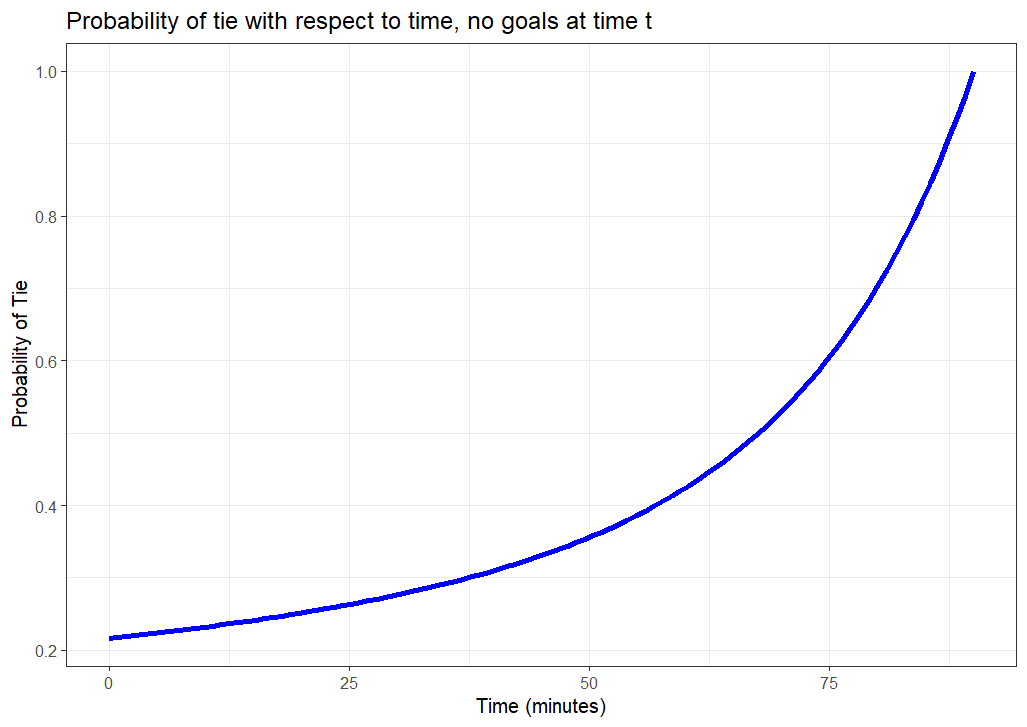
\includegraphics[width=0.7\linewidth]{tieGoalnoGoals.png}
    \caption{Probability of tie assuming at each point t, there are no goals scored yet}
\end{figure}

\textbf{c)} 

We do it with the same method as b), however, after 60 seconds we want to calculate the probability that
$N_A(t)+1 = N_B(t)$ as we now require B to score an extra goal over A. 
\[
\sum_{b=0}^{\infty}\frac{(\frac{2(90-t)}{90})^be^{-\frac{2(90-t)}{90}}}{b!}\frac{(\frac{1.5(90-t)}{90})^{b+1}e^{-\frac{1.5(90-t)}{90}}}{(b+1)!}
\]
\begin{figure}[H]
    \centering
    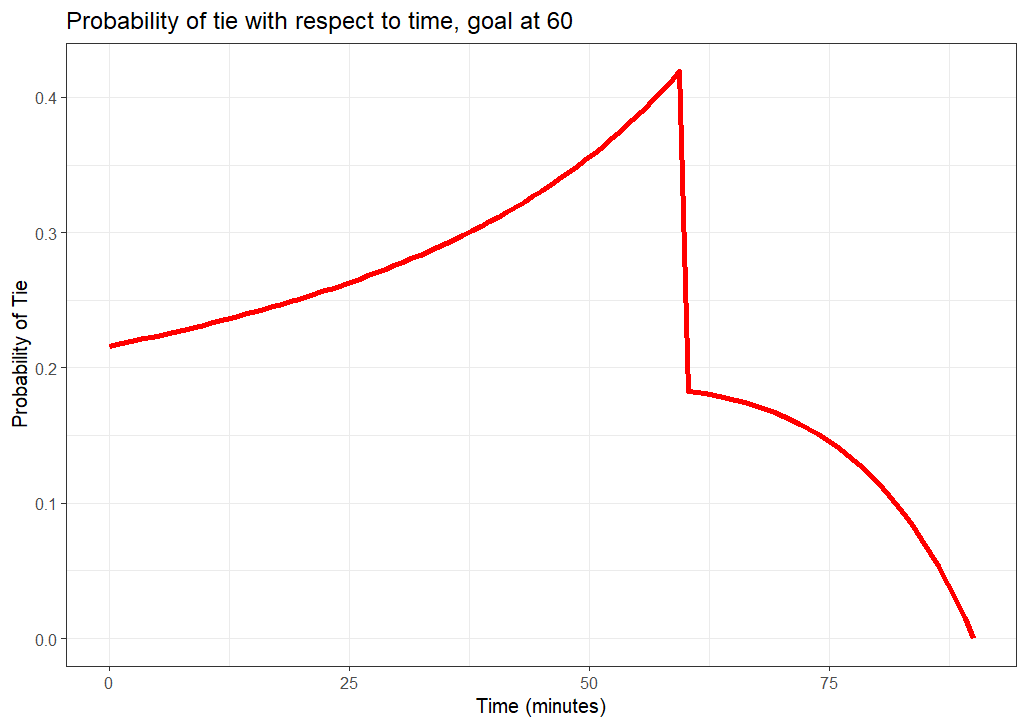
\includegraphics[width=0.7\linewidth]{tieGoalAt60.png}
    \caption{Probability, assuming a goal gets scored at 60, and no goals get scored after}
\end{figure}

\textbf{d)}

We will essentially calculate this based on the tower property:
\begin{align}
    E[A] &= \int_0^\infty E[Pois(2t/90)] 1/3e^{-t/3} dt\\
    &= \frac 1{135}\int_0^\infty te^{-t/3}dt\\
    &= \frac 1{135}(-3 te^{-t/3}-\int_0^\infty -3e^{-t/3}dt)\\
    &= \frac 1{135}(-3 te^{-t/3} - 9e^{-t/3}dt)|_0^\infty\\
    & = \frac{9}{135} = \frac 1{15} = \boxed{.0667}
\end{align}

So there is a probability of $.0074$ of scoring a goal for team A.

\section{Basketball Game} 

\textbf{a)}

For this I will be using a moment generating function, which is $\exp(\lambda(e^t-1))$
for Poisson distributions. Additionally
\[M_{(X-Y)}(s) = E[e^{(X-Y)s}]= E[e^{Xs}e^{-Ys}] = E[e^{Xs}]E[e^{-Ys}] = M_X(s)M_Y(-s)\]

We will define A as the random variable for scoring for Team A and B as a random variable for
scoring for team B.

\[
M_{A-B}(s)=\exp(t\lambda(e^s-1)+t\lambda(e^{-s}-1))
\]
\[
M_{A-B}(s)=\exp(t\lambda(e^{-s}+e^s-2))
\]

Taking the first derivative and plugging in 0 to get the expected value:
\begin{align}
    M_{A-B}'(s)|_{s=0} &= t\lambda(-e^{-s}+e^s)\exp(\lambda(e^{-s}+e^s-2))|_0\\
    &= 0 \implies 2E[A-B] = \boxed{E[D(t)] = 0}
\end{align}


Taking the second derivative to get the second moment to solve for variance:
\begin{align}
    M_{A-B}''(s)|_{s=0} &= t\lambda(e^{-s}+e^s)\exp(t\lambda(e^{-s}+e^s-2)) + 
    t\lambda(-e^{-s}+e^s)^2\exp(t\lambda(e^{-s}+e^s-2))|_0\\
    &= 2t\lambda =E[(A-B)^2]\\
    \implies Var(A-B) &= E[(A-B)^2] - E[A-B]^2 = 2t\lambda\\
    \implies 4Var(A-B) &= Var(2(A-B)) = \boxed{Var(D(t)) = 8t\lambda}
\end{align}

Or....Just do it like a normal person but sunk cost fallacy...

\textbf{b)}

So first step would be proving that this equation is actually correct following the logic from 
question 1. Note we have shown that a HPPP with rate $\lambda$ follows a poisson distribution of 
$Pois(\lambda t)$ in class.

\begin{align}
P(D(t) = 0) &= P(N_A(t) = N_B(t))\\
&=\sum_{m=0}^\infty P(N_A(t) = N_B(t)|N_B(t) = m)P(N_B(t) = m)\\
&=\sum_{m=0}^\infty P(N_A(t) = m)P(N_B(t) = m)\\
&= \sum_{m=0}^{\infty} \left[\frac{(\lambda t)^me^{-\lambda t}}{m!}\right]^2\\
&=  e^{-2\lambda t} \sum_{m=0}^\infty\frac{(\lambda t)^{2m}}{(m!)^2}\\
&=  e^{-2\lambda t} \sum_{m=0}^\infty\frac{1}{m!\Gamma(m+1)}\frac{2\lambda t}{2}^{2m}\\
&=  e^{-2\lambda t} \sum_{m=0}^\infty\frac{(2\lambda t)^{2m}}{2^{2m}(m!)^2}\\
&=  e^{-2\lambda t} I_0(2\lambda t)
\end{align}

Due to the asymptotic nature of $I_0(x) \sim e^x/\sqrt{2\pi x}$ we can approximate ties with
\[P(D(t) = 0) = \frac{1}{\sqrt{4\pi \lambda t}}\]
However we need a sufficiently large t using the equation given from wikipedia:

\[I_0(z) \sim \frac{e^{z}}{\sqrt{z}}(1+ \frac{-1}{8z}+O(z^{-2}))\]

Essentially we want to make sure that $|-1/8z| << 1$ and with the plugged in variables:

\begin{align}
    \left|\frac{-1}{16\lambda t}\right| &<< 1\\
    \frac{1}{16\lambda} &<< t\\
\end{align}

\textbf{c)}
\begin{figure}[H]
    \centering
    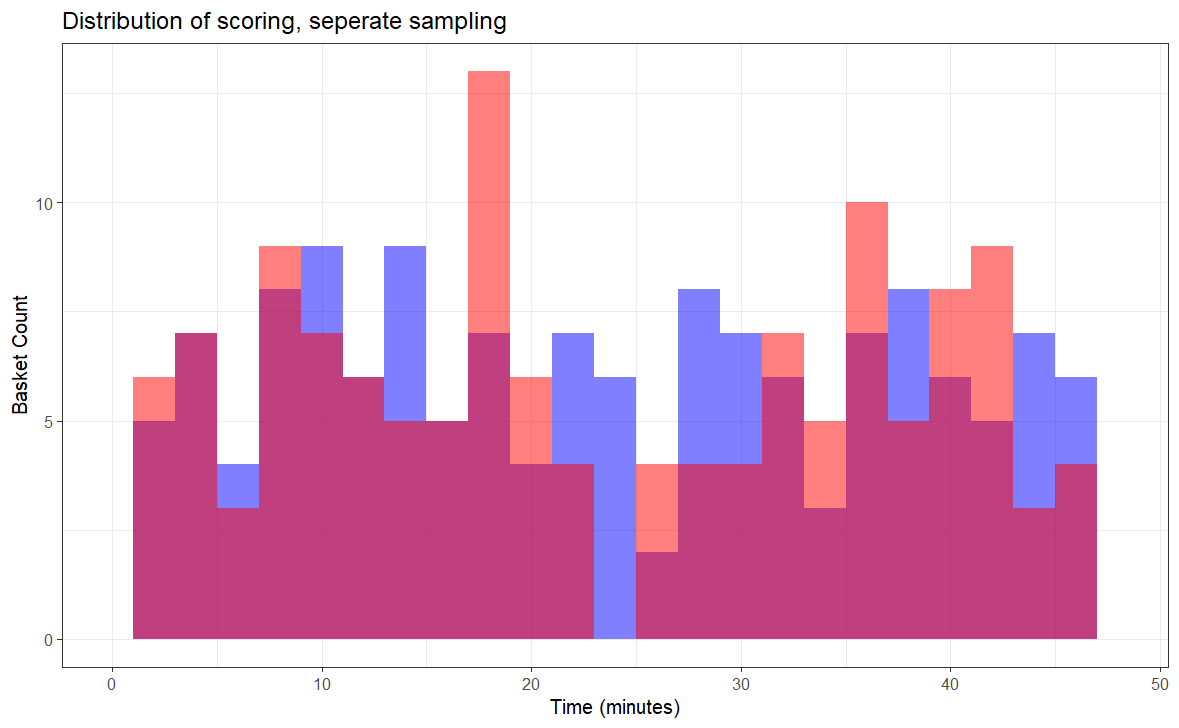
\includegraphics[width=0.7\linewidth]{seperateSampling.png}
    \caption{Scores of two teams, blue is team A and red is team B}
\end{figure}

\textbf{d)}
\begin{figure}[H]
    \centering
    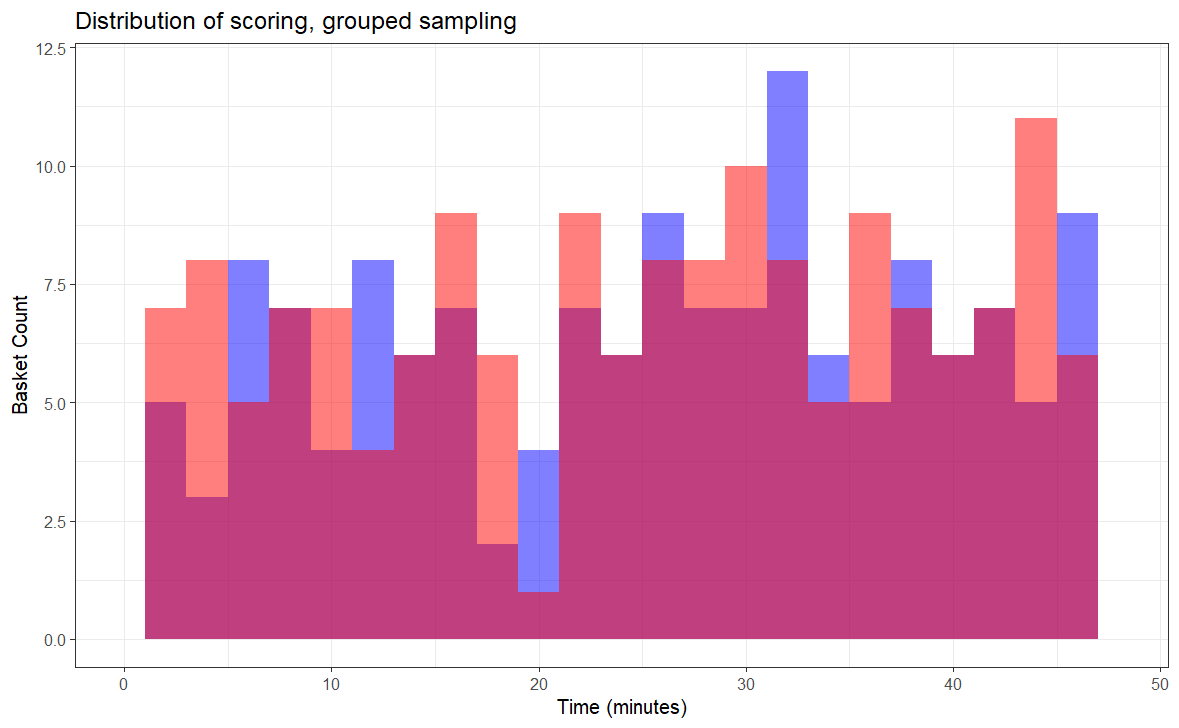
\includegraphics[width=0.7\linewidth]{groupedSampling.png}
    \caption{Scores of two teams, blue is team A and red is team B}
\end{figure}

Since the scoring is independent, we can sum up the two joint probabilities of the exponential
distribution to calculate both processes at the same time. This is simply just an addition of the
rate parameter so we sample from an exponential distribution of rate 6.

\textbf{e)}
After running the simulation we get the following estimates
\[
\begin{cases}
    E[D(48)] &= -0.3194\\
    VAR[D(48)] &= 1159.616\\
    P[D(48) = 0] &= .0227
\end{cases}
\]

This is very close the the theoretical mean of 0, theoretical variance of $1152$, and theoretical tie probability of $.0235$.
\section{Nonhomogenous Poisson Process}

\textbf{a)}

Using the given equation and say S is the number of sick students, we can calculate the probability of 
no sick students at time t.
\begin{align}
    P(S = 0)&=\exp(-\int_0^t .5(1+(t/30)^2)dt)\\
    &=\exp(-.5(t+t^3/2700)|_0^t)\\
    &=\boxed{\exp(-.5t-t^3/5400)}
\end{align}

To find the expected time of when the first case appears, we will be setting up the equation:
Also the integral does not seem like it can be evaluated analytically so it is solved through
https://www.integral-calculator.com/


\begin{align}
    P(T_1>t) = P(N(t) = 0) &= \exp(-.5t-t^3/5400)\\
    \implies \frac{d}{dt}P(t\leq T_1) = f_{T_1}(t) &= (.5+t^2/1800)\exp(-.5t-t^3/5400)\\
    \implies E[T_1] &= \int_0^\infty t(.5+t^2/1800)\exp(-.5t-t^3/5400)dt = \boxed{1.9835}
\end{align}

\textbf{b)}
To calculate the expected value of reports in 120 day we will first solve for
lambda as we also know that the expected value of a poisson distribution is lambda. 

\begin{align}
    \int_{0}^{120}\lambda(u)du &=\int_0^t .5(1+(t/30)^2)dt\\
    &=.5(t+t^3/2700)|_0^{120}\\
    &=.5(120+120^3/2700) = \boxed{380}
\end{align}

Now utilizing this lambda we know the expected value is 380 sick students.

\textbf{c)}
Note that the equation for lambda is a quadratic equation with a derivative of $t/30$, hence it is
a strictly increasing function with the maximum being the upper bound. I got a total of 389 sick people
which is pretty close to 380.

\begin{figure}[H]
    \centering
    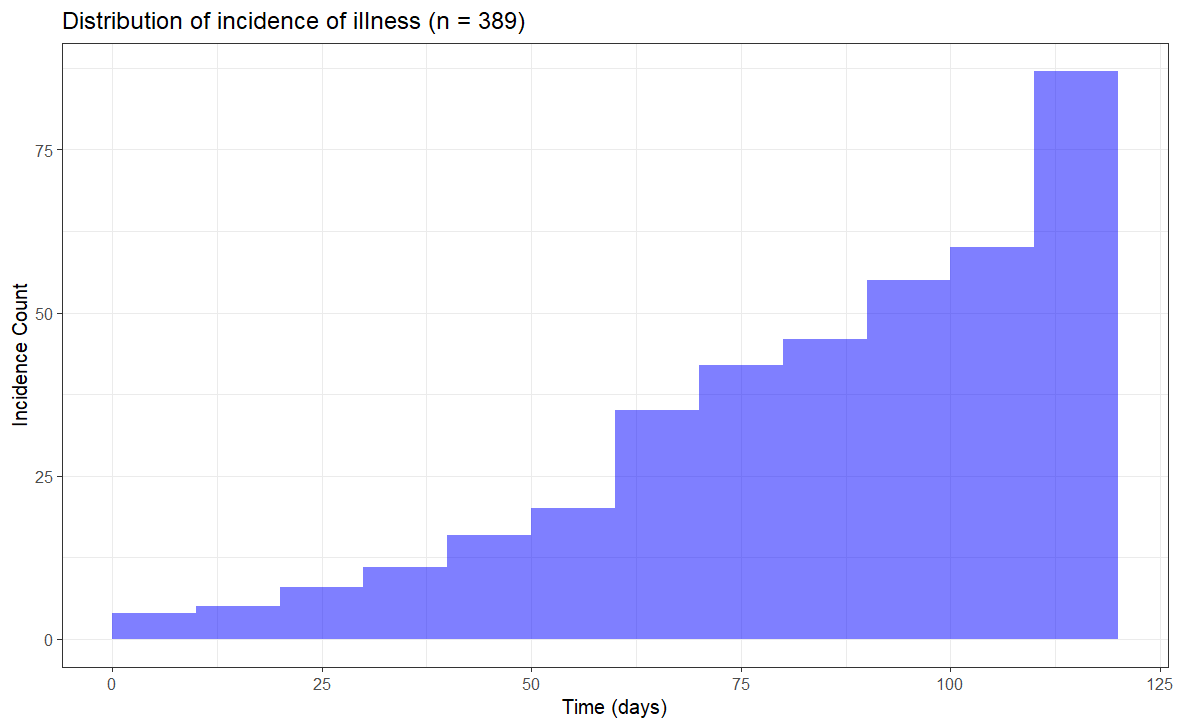
\includegraphics[width=0.7\linewidth]{distributionOfSick.png}
    \caption{Distribution of incidence of illness}
\end{figure}

\section{Arrival Time}

Essentially this is saying that we have some time t such that $T_1 \leq t < T_2$. We also know that
$ N(t) \sim Pois(t\lambda)$. I will now show that $T_1 \sim U(0,t)$. The key insight is that we know that
there must be no events between s and t.

\begin{align}
    P(T_1 \leq s|N(t) = 1) &= \frac{P(T_1 \leq s\text{ and }N(t) = 1)}{P(N(t) = 1)}, 0\leq s \leq t\\
    &= \frac{P(N(s) = 1)P(N(t)-N(s) = 0)}{\lambda t e^{-\lambda t}}\\
    &= \frac{\lambda s e^{-\lambda s} *e^{-\lambda (t-s)}}{\lambda t e^{-\lambda t}}\\
    &= \frac{\lambda s e^{-\lambda t)}}{\lambda t e^{-\lambda t}}\\
    &= \frac{s}{t}
\end{align}

Note that this is the CDF for $U(0,t)$ hence given that $N(t) = 0$ and using the fact that
increments are independent, $T_1\leq s\sim U(0,t)$

\end{document}
